\documentclass{article}
\usepackage[utf8]{inputenc}
\usepackage{tikz}
\usetikzlibrary{shapes.geometric, arrows}
\tikzstyle{startstop} = [rectangle, rounded corners, minimum width=3cm, minimum height=1cm,text centered, draw=black, fill=red!30]
\tikzstyle{io} = [trapezium, trapezium left angle=70, trapezium right angle=110, minimum width=3cm, minimum height=1cm, text centered, draw=black, fill=blue!30]
\tikzstyle{process} = [rectangle, minimum width=3cm, minimum height=1cm, text centered, draw=black, fill=orange!30]
\tikzstyle{decision} = [diamond, minimum width=3cm, minimum height=1cm, text centered, draw=black, fill=green!30]
\tikzstyle{arrow} = [thick,->,>=stealth]


\title{Deep Learning DS-GA 1008  Assignment3}

\author{Xiao Jing xj655}
\date{March 2019}

\usepackage{natbib}
\usepackage{graphicx}

\begin{document}

\maketitle

\section{Dropout}https://www.overleaf.com/project/5c86a45cbd4dbc5c7d08d4c0
\item{1. Dropout module in torch.nn}
\\
\\
\text{ m = torch.nn.Dropout2d(p=0.2)
}
Here, the skipping unit possibility is 0.2 and all
\\
\\


\item 2. What is it and Why is it useful?
The key idea is to randomly drop units (along with their connections) from the neural during the training.
network during training. 
\\
\\
This prevents units from co-adapting too much. During training,
dropout samples from an exponential number of different “thinned” networks. At test time, we just need to multiply the $w$ with probability P.

\section{Batch Norm}
\item  1. What is Mini-batch refer to deep learning?
\\
\\
Mini batch is one of the  data sets and is a portion divided from  the very large original data set.

\item 2. What is Batch Norm and why it's useful?
\\
\\
Batch normalization is to limit co-variate shift by normalizing the activation of each layer (transforming the inputs to be mean 0 and unit variance). This, supposedly, allows each layer to learn on a more stable distribution of inputs, and would thus accelerate the training of the network. Also, to make the training model working well on different distribution data.
\\
\\
Why it's useful ? If an algorithm learned some X to Y mapping, and if the distribution of X changes, then we might need to retrain the learning algorithm by trying to align the distribution of X with the distribution of Y. For example, we train our data on only black cats’ images. So, if we now try to apply this network to data with colored cats, it is obvious; we’re not going to do well. The training set and the prediction set are both cats’ images but they differ a little bit. In other words.

\section{Language Modeling}
\item (a) 
\begin{figure}[h!]
\centering
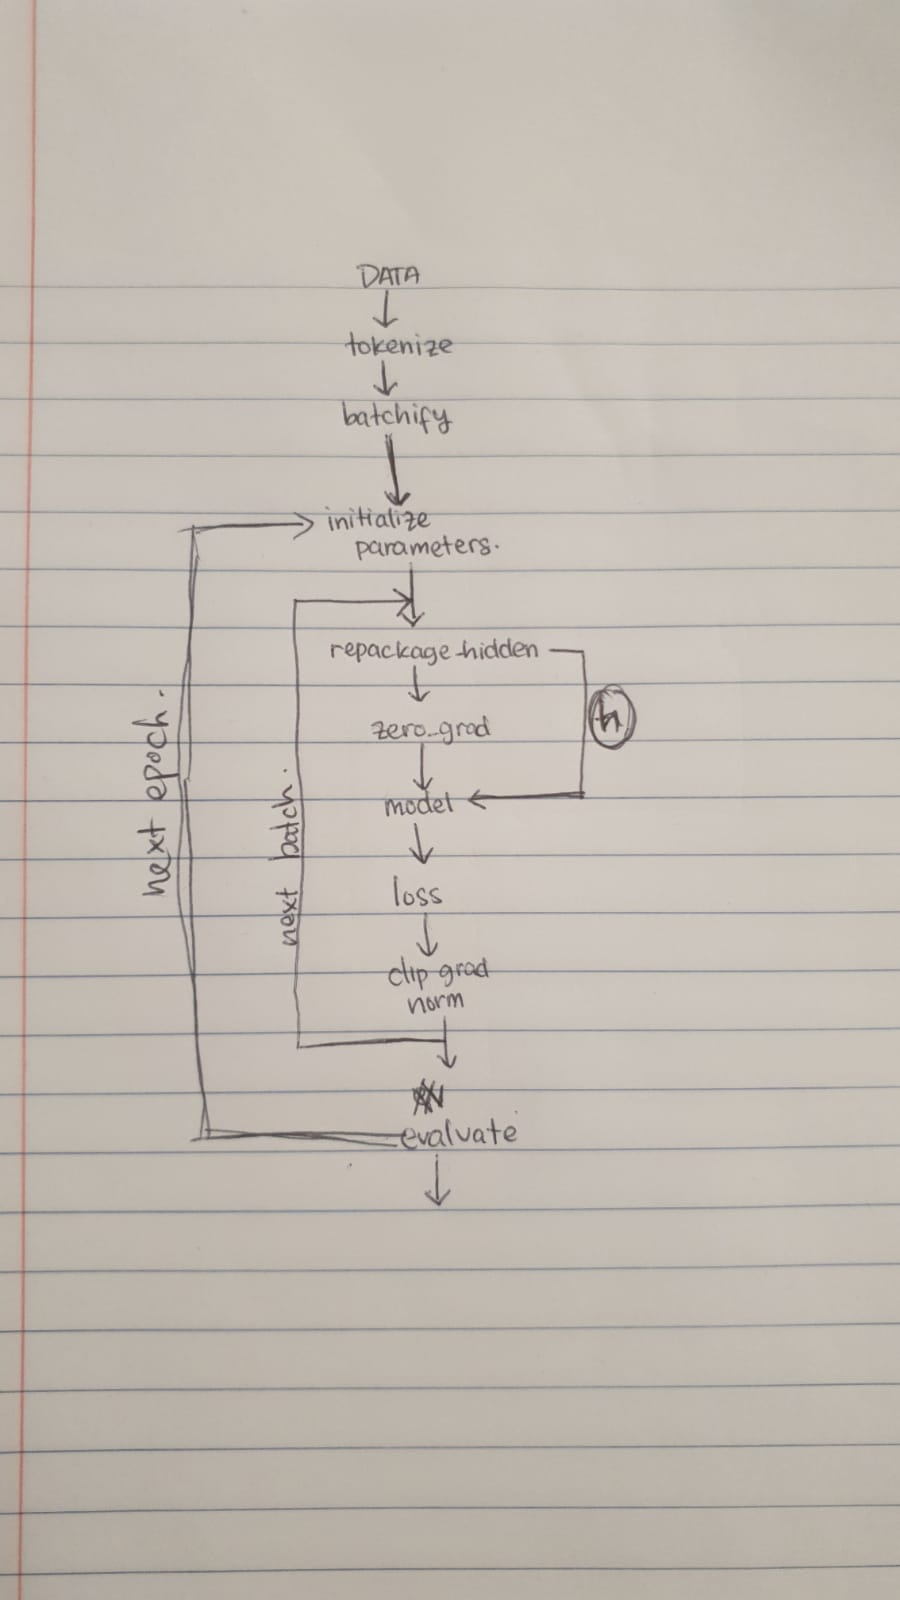
\includegraphics[scale=1.7]{flowchart}
\caption{The Flowchart}
\label{fig:universe}
\end{figure}
\\
\begin{tikzpicture}[node distance=2cm]
\node (data) [startstop] {Data input}
\node (tokenize) [startstop, below of=data] {tokenize};
\node (batchify) [process, below of=tokenize] {Intialize Parameters};
\node (ini) [startstop, below of=tokenize] {Intialize Parameters};
\node (repackage-hidden) [decision, below of=ini, yshift=-0.5cm] {repackage-hidden};
\node (zero-grad) [startstop, below of=repackage-hidden, yshift=-0.5cm] {zero-grad};
\node (model) [startstop, right of=zero-grad] {model};
\node (loss) [startstop, right of=zero-grad]{loss};
\node (grad-norm) [startstop, below of=loss] {grad-norm};
\node (e) [startstop, below of=grad-norm] {evaluate};
\node (out) [startstop, below of=e] {output};
\node (next-batch) [startstop, left of=model] {next batch};
\node (next-epoch) [startstop, left of=loss] {next epoch};
\node (h) [startstop, right of=zero-grad] {hidden};

\draw [arrow] (data) -- (tokenize);
\draw [arrow] (tokenize) -- (ini);
\draw [arrow] (batchify) -- (ini);
\draw [arrow] (ini) -- (repackage-hidden);
\draw [arrow] (repackage-hidden) -- (zero-grad);
\draw [arrow] (zero-grad) -- (model);
\draw [arrow] (model) -- (loss);
\draw [arrow] (loss) -- (grad-norm);
\draw [arrow]  (grad-norm) --(e);
\draw [arrow]  (e) --(out);

\draw [arrow] (e) |- node[anchor=east] {next batch} (repackage-hidde);
\draw [arrow] (grad-norm) |- node[anchor=south] {each epoch} (ini);
\draw [arrow] (pro2b) |- (pro1);


\end{tikzpicture}

\item (b) 
\\
\\
During each  train function to train each batch size sequence, the loss.backward() in line 159 is to BPTT process, using the critieria of nn.CrossEntropyLoss to find the gradient descent. Iterate training the sequence and each time use backprop to increase the model. 
\item (c) 
\\
\\
Wrap hidden states in new Variables, to detach them from their history. In each evaluate and each training, the hidden will be repackaged.

\item (c) 
\\
\\
1. One-hot encoded vectors are high-dimensional and sparse. In a big dataset this approach is not computationally efficient.
\\
2. High similarities between words will be found in a multi-dimensional space. Embedding allows us to visualize relationships between words, but also between everything that can be turned into a vector through an embedding layer.

\item (d)  This work is  a collaberate work, I and my team member train a model and share the model result
\\
\\
LSTM Epoch 20: time 46.05s | test ppl   116.47
\\
GRU Epoch 20: time: 27.60s | test ppl    150.20
\\
LSTM Epoch 40: time 46.05s | test ppl   109.57
\\
GRU Epoch 40: time 27.31s  | test ppl 145.92
\\
LSTM bptt 35: time 48.06s | test ppl   109.57
\\
GPU bptt 35: time 39.19s | test ppl   134.87
\\
LSTM bptt 50: time 41.68s  | test ppl   107.40
\\
GRU bptt 50: time 38.72s | test ppl 114.85
\\
LSTM emsize 100: time 28.03s | test ppl  108.89
\\
GRU emsize 100: time: 38.38s| test ppl   218.64
\\
LSTM emsize 200: time 28.55s | test ppl   107.58
\\
GRU emsize 200: time 39.12s  | test ppl 134.87

As to epoch, GRU just finished more quickly, but more perplexity\\

As to bptt, GPU run faster, but more perplexity\\

As to emsize, GPU run slower, and also more perplexity
\item (e)
\\
\\
To give a good effective test score otherwise, each loss will be the same
\end{document}
